%%%%%%%%%%%%%%%%%%%%%%%%%%%%%%%%%%%%%%%%%%%%%%%%%%%%%%%%%%%%%%%%%%%%%%%%%%%%%%%%
%2345678901234567890123456789012345678901234567890123456789012345678901234567890
%        1         2         3         4         5         6         7         8

\documentclass[letterpaper, 10 pt, conference]{ieeeconf}  % Comment this line out if you need a4paper

%\documentclass[a4paper, 10pt, conference]{ieeeconf}      % Use this line for a4 paper

\IEEEoverridecommandlockouts                              % This command is only needed if 
                                                          % you want to use the \thanks command

\overrideIEEEmargins                                      % Needed to meet printer requirements.

%In case you encounter the following error:
%Error 1010 The PDF file may be corrupt (unable to open PDF file) OR
%Error 1000 An error occurred while parsing a contents stream. Unable to analyze the PDF file.
%This is a known problem with pdfLaTeX conversion filter. The file cannot be opened with acrobat reader
%Please use one of the alternatives below to circumvent this error by uncommenting one or the other
%\pdfobjcompresslevel=0
%\pdfminorversion=4

% See the \addtolength command later in the file to balance the column lengths
% on the last page of the document

% The following packages can be found on http:\\www.ctan.org
%\usepackage{graphics} % for pdf, bitmapped graphics files
%\usepackage{epsfig} % for postscript graphics files
%\usepackage{mathptmx} % assumes new font selection scheme installed
%\usepackage{times} % assumes new font selection scheme installed
\usepackage{amsmath} % assumes amsmath package installed    
\usepackage{amssymb}  % assumes amsmath package installed
\usepackage{url}
\usepackage{float}
\usepackage{graphicx}
\usepackage{algorithm,algpseudocode}

\title{\LARGE \bf
PMorph: A Task-Specialized Robot Manipulator Morphology Optimizer 
}


\author{Stephen Gillet$^{1}$% <-this % stops a space
\thanks{*This work was not supported by any organization}% <-this % stops a space
\thanks{$^{1}$Stephen Gillet is a Master's student with the Robotic Program,
        University of Colorado Boulder, Boulder, CO 80309, U.S.A.
        {\tt\small stgi5837@colorado.edu}}%
}


\begin{document}



\maketitle
\thispagestyle{empty}
\pagestyle{empty}


%%%%%%%%%%%%%%%%%%%%%%%%%%%%%%%%%%%%%%%%%%%%%%%%%%%%%%%%%%%%%%%%%%%%%%%%%%%%%%%%
\begin{abstract}

This paper seeks to address the overactuation, energy-ineffiency, and lack of task specialization seen in manufacturing from the current suite of generalized robotic manipulators.
The approach involves specifying a task in a MuJoCo simulated environment and then using a PPO agent to optimize the morphology for that enviroment given a reward function.
The morphological elements to be optimized include the number of links, the lengths of each link, and the type of joints involved.
The reward function is tuned to weigh energy cost, end effector movement, end effector accuracy, manipulability measures, number of links, and task completion.
PPO is ideal for this task because it can efficiently optimize over the continuous action space that is morphology, resulting in a robot that is more simple, efficient, and capable than those commonly used in industry today. 

\end{abstract}


%%%%%%%%%%%%%%%%%%%%%%%%%%%%%%%%%%%%%%%%%%%%%%%%%%%%%%%%%%%%%%%%%%%%%%%%%%%%%%%%
\section{Introduction}

Imagine a factory where every employee has to be trained on and work every job in the plant.
Imagine how inefficient that would be.
Every employee would have general knowledge and ability, but no one would have a chance to specialize and become very good at any particular job.
This is exactly the state of robotics in manufacturing today where high costs and lack of tailorability are some of the most cited problems for the adoption of robotics \cite{mckinsey2019industrial}\cite{patel2024}.
To make matters worse \cite{russo2021task} and \cite{he2019underactuated} show that most manipulators are overactuated, inefficient, and ineffective for most tasks they are used in today.

This paper seeks to address these issues by using a PPO agent to optimize the morphology of a robotic manipulator to the particular task it is being used for.
This ensures that the robot is as simple, efficient, and capable as possible for its particular job while still allowing the designer to specify the level of robustness.

PPO was chosen for its ability to explore the continuous action space that is morphology and it has been shown to do so efficiently and robustly \cite{schulman2017proximal}.
The core method is to use Stable Baselines3 PPO implementation to iterate on the design parameters (number of links, joint types (X, Y, Z hinge, and Z actuation), and link lengths), use MuJoCo to simulate that iteration on a simple task using RRT-Connect and damped least squares (DLS) inverse kinematics (IK) for the path planning, feed the results (success, efficiency, and manipulability index) back into the PPO model.
RRT-Connect was chosen for simplicity and it has been shown to be faster than other methods \cite{kuffner2000rrt} which enables faster and more robust training.
DLS IK was chosen for a similar reason, it has been shown to be robust especially in situations where the target position is out of reach \cite{buss2004introduction} which is inevitable when exploring morphologies, some of which will be too small or otherwise poorly suited to the task as the agent learns.

The evaluation signals will be successful path planning, path length, energy cost, and manipulability index.
The manipulability index is a measure of a manipulators ability to arbitrarily change the position and orientation of the end effector at a particular point, borrowed from \cite{yoshikawa1985manipulability}.
The tasks will be kept simple but varied in ways to test different types of movements like moving near the base, moving from near to far, different elevations, more linear movements, and different obstacle contraints.
One might imagine that a lot of pick and place tasks are mostly linear and so might largely be done by linear actuators more efficiently for example.

The research questions to be answered: Can PPO be used to generate more efficient morphologies? Can morphologies be generated for tasks that generalized manipulators cannot do or cannot perform well? Can more simple morphologies (less DOF) be generated that can perform the same tasks with similar levels of accuracy?

\section{Related Work}

Most of the research in this area codesigns morphology and control of atomic, modular robots. 
\cite{bhatia2023reinforcement} shows that PPO can be used to generate freeform morphologies optimized for locomotion tasks from a set of atomic modules.
\cite{tjanaka2023co} shows that reinforcement learning can be used on a modular robot to co-optimize morphology and control and outperform optimized control on a fixed morphology. 
\cite{spielberg2025accelerated} also uses reinforcement learning to co-optimize with the addition of a pretrained foundation model to accelerate the training process and improve results.

Most pertinently to this paper, \cite{kalimuthu2023} shows that PPO and A3C can be used to generate optimal morphologies that improve performance of reconfigurable robots,
\cite{ding2024modular} uses DDQN to co-optimize morphology and control for modular robotic manipulators, and \cite{luck2019data} uses soft actor critic for co-optimization showing that the approach resulted in drastically less design prototypes.
This background motivates the approach of this paper which is going to use simple controllers and similar reinforcement learning techniques to maximize morphological potential.
FANUC 6-DOF series of manipulators are the most commonly used in industry today \cite{patentpc2025toprobotics}\cite{standardbots2025fanucprice} and so their morphology will be used as a baseline for comparison.
Given the same environment, task, and controllers which morphologies will perform better?

\section{Problem Formulation}

The task is formulated as a single-step reinforcement learning problem in a MuJoCo simulated environment.
A morphology $\theta$ is chosen, run through the simulation, and then evaluated based on weighted reward function terms.

\subsection{Morphology Parameterization}

A candidate morphology is defined by the tuple
\[
\theta = (n, l, j),
\]
where
\begin{itemize}
    \item $n \in \{2, \dots, 7\}$ is the number of links,
    \item $l = [l_1, \dots, l_n] \in [0.05, 1.2]^n$ are the link lengths (m),
    \item $j = [j_1, \dots, j_n] \in \{0,1,2,3\}^n$ are the joint types (0: revolute about x, 1: about y, 2: about z, 3: slide in z).
\end{itemize}
The action space of the RL agent is the continuous box
\[
\mathcal{A} = [0,1]^{1 + 7 + 7},
\]
from which $n$, $l$, and $j$ are decoded.

\subsection{Task Specification}

The robot has to move from start poses to goal poses (position + unit quaternion) in a cluttered workspace with fixed obstacles (walls, shelves, ceilings).
An example of such an environment may be seen in Figure \ref{fig:containerTask}, which shows the container task where two sets of start and goal poses are set at either ends of a shipping-container-like workspace with the arm positioned in the middle.
The poses are modified with Gaussian noise ($\sigma=0.05$) at evaluation in order to encourage robust designs.

\begin{figure}[H]
  \centering
  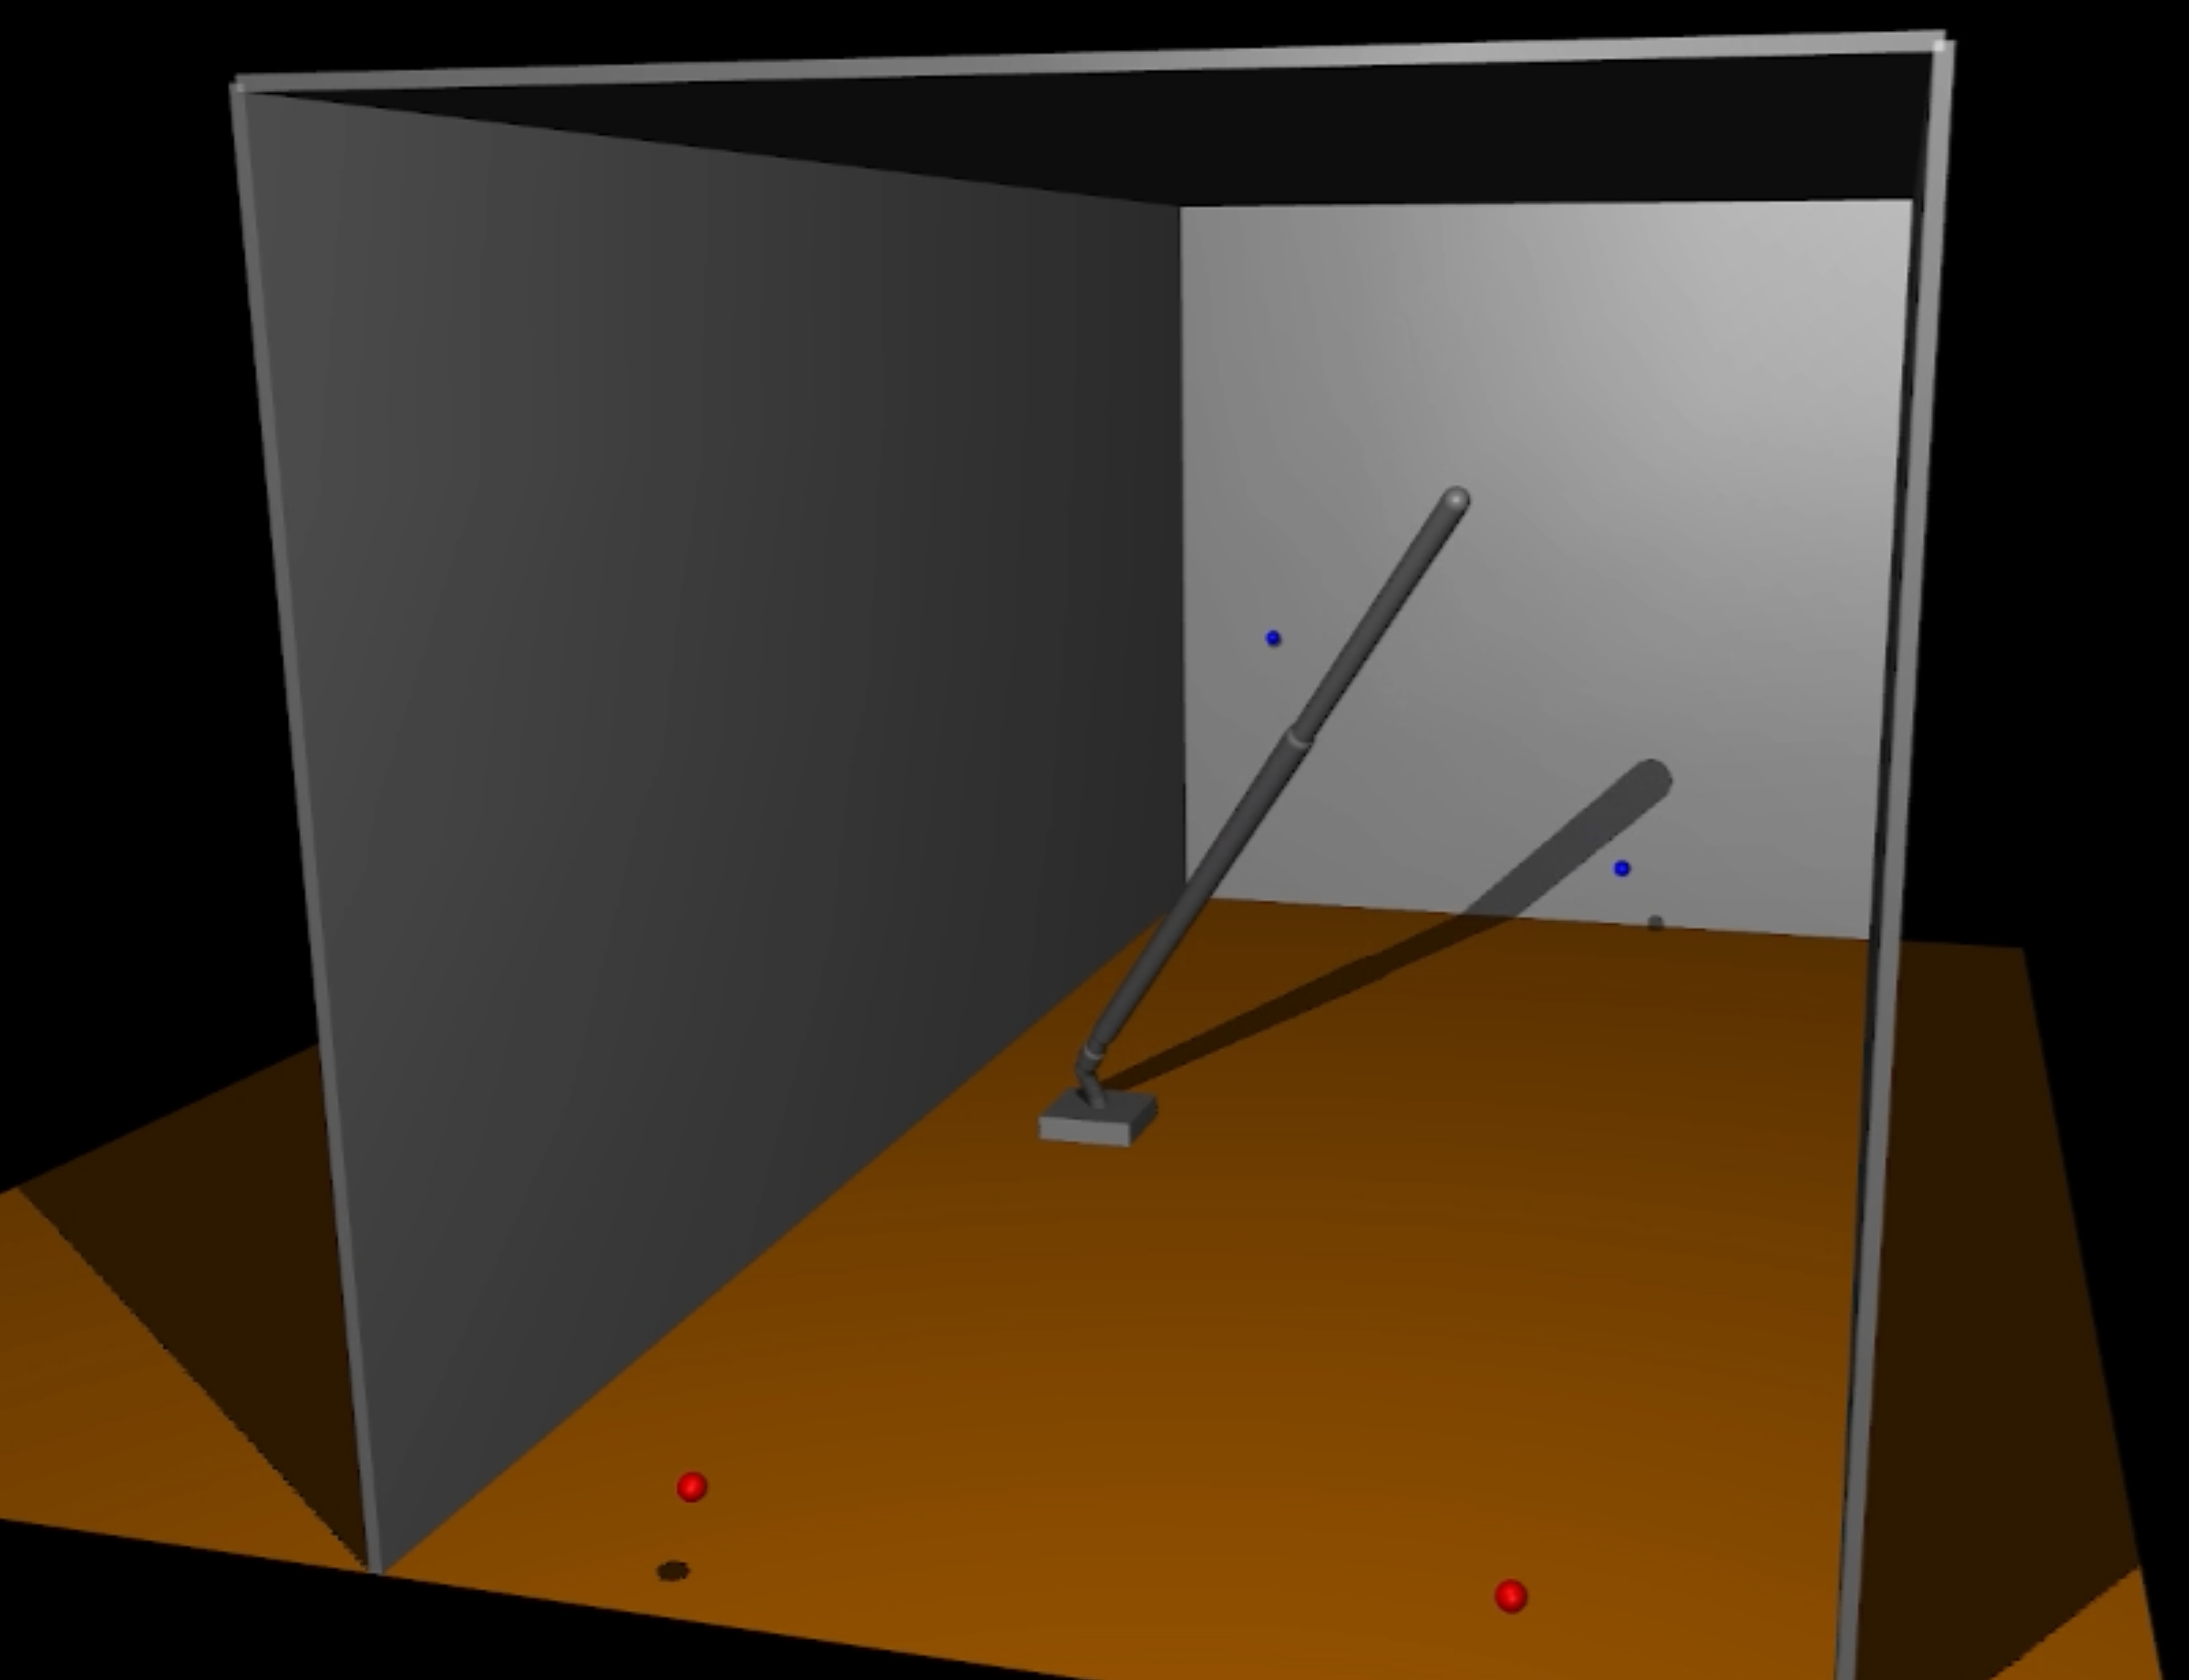
\includegraphics[width=0.9\columnwidth]{containerTask.png}
  \caption{Container task. Start and goal positions represented with blue and red dots surrounded by wall and ceiling obstacles.}
  \label{fig:containerTask}
\end{figure}

\subsection{Evaluation Pipeline}

Morphology $\theta$ is evaluated as follows:
\begin{enumerate}
    \item A MuJoCo XML model is generated with $\theta$ and the task poses/obstacles.
    \item Inverse Kinematics is solved for the start and goal poses using Damped Least Squares.
    \item A path between the start and goal configurations is computed using RRT-Connect.
    \item If a path connect be found, return reward $30 - 100 \times \text{IK error}$.
    \item Otherwise, calculate the other reward terms and return the weighted sum:
    \begin{itemize}
        \item End-effector path length $p = \sum \|\mathbf{x}_{ee}^{t+1} - \mathbf{x}_{ee}^t\|$ (Euclidean distance between each point along path),
        \item Manipulability $\mu = \min(\sigma(\mathbf{J}))$ (minimum singular value of manipulability jacobian at start and goal \cite{klein1987dexterity}),
        \item Energy $E = \sum \|\boldsymbol{\tau} \odot \mathbf{v}\| \cdot \Delta t$ (MuJoCo inverse dynamics using constant velocity segments along path at torque limits).
    \end{itemize}
\end{enumerate}

\subsection{Reward Function}

The scalar reward is
\begin{align}
r(\theta) &= \frac{1}{N} \sum_{i=1}^{N} \Biggl[ 
    w_0 \cdot \text{success}_i 
    - w_1 \cdot p_i \notag \\
    &\quad - w_2 \cdot (e_{\text{start},i} + e_{\text{goal},i}) 
    + w_3 \cdot (\mu_{\text{start},i} + \mu_{\text{goal},i}) \notag \\
    &\quad - w_4 \cdot (n - 2) 
    - w_5 \cdot E_i 
\Biggr]
\label{eq:reward}
\end{align}
where $N$ is the number of start–goal pairs, $e$ is IK error, success is valid path, and the weights ($w_k$) are tuned to balance the competing objectives (accuracy vs. efficiency vs. manipulability). 
The final optimization problem is therefore
\[
\theta^* = \arg\max_{\theta} \mathbb{E}_{\pi(\cdot|\phi)} \bigl[ r(\theta) \bigr],
\]
where $\pi$ is the PPO policy given the parameters $\phi$.

This formulation encodes the challenges outlined in Section 1:
\begin{enumerate}
    \item Energy efficiency via the energy term.
    \item Task specialization via the success, accuracy, and manipulability terms.
    \item And simplicity via the link number and path length terms.
\end{enumerate}

\section{Method}

\subsection{PPO Action Decoding}

The PPO agent selects an action $a \in [0,1]^{15}$ which is then decoded into morphology parameters $\theta$ as shown in Algorithm \ref{alg:decode}.

\begin{algorithm}[H]
\caption{Morphology Decoding from PPO Action}
\label{alg:decode}
\begin{algorithmic}[1]
\State \textbf{Input:} action \(a \in [0,1]^{15}\)
\State \(n \gets \text{round}(a_0 \cdot (7-2) + 2)\) \Comment{links: 2--7}
\State \({l} \gets a_{1:8} \cdot (1.2 - 0.05) + 0.05\) \Comment{lengths (m)}
\State \({j} \gets \text{round}(a_{8:15} \cdot 3)\) \Comment{types: 0--3 (hinge X/Y/Z, slide Z)}
\State \textbf{Return:} \(\theta = (n, {l}_{:n}, {j}_{:n})\)
\end{algorithmic}
\end{algorithm}

\subsection{Simulation}

$\theta$ is then passed into the evaluation environment, which is implemented as a Gymnasium class `robotArmEnv'.

\begin{enumerate}
    \item \textbf{XML Generation}: A dynamic MuJoCo model is built via `generateXML($n$, $l$, $j$)', which assembles the links sequentially according to the parameter specifications using revolute/slide joints and capsule geoms (mass = $l_i$). Fixed obstacles (walls, ceiling, shelves, floor) are included as per the task set up.
    \item \textbf{Path Planning}: Damped least-squares IK (robust variant with collision-aware line search) solves for start/goal configurations. RRT-Connect then finds a collision-free joint-space path \cite{kuffner2000rrt}, using constant-velocity segments for energy estimation via MuJoCo inverse dynamics.
    \item \textbf{Reward Computation}: \(r(\theta)\) from Eq.~\eqref{eq:reward} is returned with \(N\) being the number of sets of start and goal poses in the task and noise (\(\sigma=0.05\)) added to poses for robustness.
\end{enumerate}

\subsection{Training}

Training follows the standard PPO loop over 1M timesteps (single-step episodes):

\begin{algorithm}[H]
\caption{PMorph Training}
\label{alg:train}
\begin{algorithmic}[1]
\State Initialize PPO policy \(\pi_\phi\)
\For{each episode \(t = 1\) to 1M}
    \State Sample \(\theta \sim \pi_\phi(\cdot|\phi)\)
    \State \(r \gets \texttt{eval}(\theta)\) \Comment{Section FILLIN}
    \State Store \((\theta, r)\) in buffer
    \State Update \(\phi\) via the clipped surrogate loss \cite{schulman2017proximal}:
    \[
    \begin{aligned}
    \mathcal{L}(\phi) &= \hat{\mathbb{E}}_t \Bigl[ 
        \min\bigl( r_t(\phi) \hat{A}_t,\; \\
        &\quad \text{clip}\bigl(r_t(\phi), 1-\epsilon, 1+\epsilon\bigr) \hat{A}_t \bigr) \Bigr] \\
        &\quad + S[\pi_\phi](s_t) - \beta \cdot \mathbb{E}_t \bigl[ (\hat{V}_\phi(s_t) - V_t^{\text{targ}})^2 \bigr]
    \end{aligned}
    \]
    \Comment{\(\epsilon=0.2\), GAE advantages \cite{schulman2015high}}
\EndFor
\end{algorithmic}
\end{algorithm}

Hyperparameters: \(\epsilon=0.2\) (clip ratio) and \(\beta=0.5\) (value loss weight)

\subsection{Evaluation}

After training, the optimized morphology \(\theta^*\) is evaluated on a test set of start/goal pairs with noise.
The reward terms are averaged over that test set to assess performance.
A comparison is made using the baseline FANUC-like arm morphology.
Based on the most commonly used model (FANUC LR Mate 200iD \cite{fanuc2024lrmate}), the baseline has 6 links, with lengths of 0.165, 0.330, 0.08, 0.285, 0.05, 0.05 (meters), and joint types of 2, 0, 0, 2, 0, 2 (revolute about z, x, x, z, x, z).

\section{CONCLUSIONS}

A conclusion section is not required. Although a conclusion may review the main points of the paper, do not replicate the abstract as the conclusion. A conclusion might elaborate on the importance of the work or suggest applications and extensions. 

\addtolength{\textheight}{-12cm}   % This command serves to balance the column lengths
                                  % on the last page of the document manually. It shortens
                                  % the textheight of the last page by a suitable amount.
                                  % This command does not take effect until the next page
                                  % so it should come on the page before the last. Make
                                  % sure that you do not shorten the textheight too much.

%%%%%%%%%%%%%%%%%%%%%%%%%%%%%%%%%%%%%%%%%%%%%%%%%%%%%%%%%%%%%%%%%%%%%%%%%%%%%%%%



%%%%%%%%%%%%%%%%%%%%%%%%%%%%%%%%%%%%%%%%%%%%%%%%%%%%%%%%%%%%%%%%%%%%%%%%%%%%%%%%



%%%%%%%%%%%%%%%%%%%%%%%%%%%%%%%%%%%%%%%%%%%%%%%%%%%%%%%%%%%%%%%%%%%%%%%%%%%%%%%%
\section*{APPENDIX}

Appendixes should appear before the acknowledgment.

\section*{ACKNOWLEDGMENT}

The preferred spelling of the word "acknowledgment" in America is without an "e" after the "g". Avoid the stilted expression, "One of us (R. B. G.) thanks . . ."  Instead, try "R. B. G. thanks". Put sponsor acknowledgments in the unnumbered footnote on the first page.



%%%%%%%%%%%%%%%%%%%%%%%%%%%%%%%%%%%%%%%%%%%%%%%%%%%%%%%%%%%%%%%%%%%%%%%%%%%%%%%%

References are important to the reader; therefore, each citation must be complete and correct. If at all possible, references should be commonly available publications.



\bibliographystyle{IEEEtran}
\bibliography{references}

\end{document}
